\documentclass[12pt,a4paper]{report}

%%% User pakcages

\usepackage[font=scriptsize]{caption} %small caption text
\usepackage{wrapfig}
\usepackage{afterpage}
\usepackage{parskip} % Disable US-type paragraph
\usepackage{amsfonts} % Math 
\usepackage{palatino} % Vektor fonts
\usepackage{mathptmx}
\usepackage[T1]{fontenc} 
\usepackage[utf8]{inputenc} %%\usepackage[utf8x]{inputenc} 
\usepackage{float}
\usepackage[danish]{babel} % Danish letters 
\usepackage{booktabs} % Nice tabels
\usepackage[pdftex]{graphicx} % Include graphics 
\usepackage{fancyhdr} % header & footer
\usepackage[hyphens]{url}
\usepackage[hidelinks, breaklinks]{hyperref} % Hyper link
\PassOptionsToPackage{hyphens}{url}\usepackage{hyperref}
\usepackage{titlesec}
\usepackage{xfrac}
\usepackage{listings} % Insert code
\usepackage[usenames,dvipsnames,svgnames,table]{xcolor}


\usepackage[backend=bibtex]{biblatex}
\bibliography{Kilder/kilder.bib}
\usepackage[left=2.5cm,right=2.5cm,top=2.5cm,bottom=2.5cm]{geometry} % Page margin
\usepackage{tabularx} % Table
\usepackage{marginnote}

\titleformat{\chapter}{\normalfont\huge\bfseries}{ \thechapter.}{20pt}{\huge}
\setcounter{section}{0}
\pagestyle{fancy}
\fancypagestyle{arabic}
{
    \fancyhf{}
    \setlength{\headheight}{15pt}
}

\renewcommand{\chaptermark}[1]{ \markboth{#1}{} }
\fancypagestyle{chp}{
  \fancyhf{}
  \rhead{\rightmark}%\colorbox{black}{\color{white}{\rightmark}}}
  \cfoot{\thepage}
}

\pagestyle{chp}

\title{Ground Handling}
\author{
    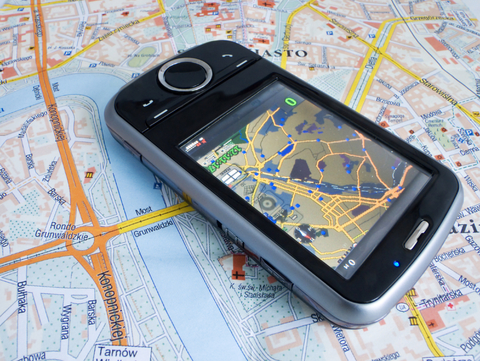
\includegraphics[width=14cm]{grafik/index} \\
        Kasper Ø. Helsted, Jens H. Stærmose, Christoffer C. Christensen, Christian H. Nielsen\\
        Kasper F. Christensen, Anders L. Matthiassen \& Josias Laugesen\\
}
\date{21 - 05 - 2014}

\definecolor{codecomment}{HTML}{383838}

\lstset{language=C,
    basicstyle=\ttfamily\scriptsize,
    keywordstyle=\color{Blue}\ttfamily,
    otherkeywords={WIDTH},
    keywords=[2]{__shared__},
    keywordstyle=[2]\color{orange}\ttfamily,
    stringstyle=\color{red}\ttfamily,
    commentstyle=\color{codecomment}\ttfamily,
    breaklines=true,
    numbers=left,
}

\begin{document}
    \maketitle
    \afterpage{\null\newpage}
    \pagenumbering{gobble}
    \clearpage  
    %Titlepage 
    \thispagestyle{empty}
\begin{titlepage}
	\setlength{\textwidth}{15cm}
	\noindent
	\begin{nopagebreak}
		{\samepage 
			\begin{tabular}{lr}
				\parbox{0.5\textwidth}{\raisebox{11mm}
					{
\includegraphics[height=1.2cm]{Grafik/aauLogoDa}}
				} &
				\parbox{0.5\textwidth}{
					\small
					\begin{tabular}{l}
						{\sf\small \textbf{Institute of Computer Science}}\\
						{\sf\small Strandvejen 12-14, 9000 Aalborg} \\
						{\sf\small Telephone 96 35 97 31} \\
						{\sf\small Fax 98 13 63 93} \\
						{\sf\small http://tnb.aau.dk}
					\end{tabular}
				}
			\end{tabular}
			
			\noindent
			\begin{tabular}{cc}
				\parbox{7cm}{
					\begin{description}
			
						\item {\bf Title:} 
			
							\textbf{Ground Handling}\\
						\item {\bf Project Period:}\\
			  				Spring Semester 2014\\
			 				\hspace{4cm}
						\item {\bf Project Group:}\\
							SW2-A418\\
			  				\hspace{4cm}
						\item {\bf Participants:}\\
							Kasper Østergaard Helsted\\
                            Jens Hegner Stærmose\\
                            Christoffer Carlé Christensen\\
                            Christian Heider Nielsen\\
                            Kasper Fuglsang Christensen\\
                            Anders Lykke Matthiassen\\
                            Josias Laugesen\\
							\hspace{2cm}
						\item {\bf Supervisor:}\\
							Ramin Sadre\\

						\item {\bf Copies:}\\ 10\\
						\item {\bf Page Numbers:}\\ 65\\
						\item {\bf Appendix:}\\ None\\
						\item {\bf Number and Type of Annexes:}\\ 14 pages, code\\
						\item {\bf Date of Completion:}\\ 21-05-2014\\
					\end{description}
					\vfill
				} &
				\parbox{7cm}{
					\vspace{.15cm}
					\hfill 
					\begin{tabular}{l}
						{\bf Abstract:}\bigskip \\
						\fbox{
							\parbox{6.5cm}{\smallskip
								{\vfill{\small \section* {Synopsis}

								\smallskip}}
							}
						}
  					\end{tabular}
  				}
			\end{tabular}
		}\\
		\\
		\noindent{\footnotesize\emph{The content of this report is freely accessible, but publication (with referencing) may only happen under agreement with the authors.}}
	\end{nopagebreak}
\end{titlepage}

    \afterpage{\null\newpage}
    \pagenumbering{gobble}
    \clearpage  
    \pagenumbering{roman}
    \chapter*{Forord}


    \renewcommand*\contentsname{Indholdsfortegnelse}
    \tableofcontents
    \thispagestyle{empty}
    \pagenumbering{arabic}
    \clearpage
    \setcounter{page}{1}
	
    \part{Problemanalyse}

    \section{In case of an emergency}

Occasionally an unexpected emergencies at airport incurs, the airport needs to respond to. A standard service manual for handling potential emergencies exists, for the relevance of this project it is interesting to know how to handle and maintain emergency landings. Which runway to shut down and prepare for the emergency, how to handle incoming and outgoing traffic and other airport services.
The manual suggest following plan for an aircraft accident on the airport:



In general alot of different (organisations / agencies) is involved in these emergencies, each with their own responsibilities. The airport traffic services includes following:

\begin{quotation}
Chapter 4
RESPONSIBILITY AND ROLE OF EACH AGENCY FOR EACH TYPE OF EMERGENCY

4.1 AIRCRAFT ACCIDENT ON THE AIRPORT
4.1.1 General
The airport emergency plan shall be implemented immediately upon an aircraft accident occurring on the airport. For this
type of emergency, responding agencies are expected to take action as described in 4.1.2 to 4.1.10 below.
4.1.2 Action by air traffic services
4.1.2.1 Initiate emergency response by using the crash alarm communication system (See Figure 8-1).
4.1.2.2 Notify the rescue and fire fighting service and provide information on the location of the accident, grid map
reference and all other essential details, including time of the accident and type of aircraft. Subsequent notification may
expand this information by providing details on the number of occupants, fuel on board, aircraft operator, and any
dangerous goods on board, including quantity and location, if known.
4.1.2.3 Close the affected runway and minimize vehicle traffic on that runway to prevent disturbance of accident
investigation evidence (See 4.1.5 2) f)).
4.1.2.4 If required, initiate communications to the police and security services, airport authority, and medical
services in accordance with the procedure in the airport emergency plan. Provide the contacts with grid map reference,
rendezvous point and/or staging area and airport entrance to be used.
4.1.2.5 Issue the following Notice to Airmen (NOTAM) immediately:
“Airport rescue and fire fighting service protection unavailable until (time) or until further notice. All equipment committed
to aircraft accident.”
4.1.2.6 Verify by written checklist that the actions above were completed, indicating notification time(s) and name
of person completing action.



4.3 FULL EMERGENCY
4.3.1 General
The agencies involved in the airport emergency plan shall be alerted to “full emergency” status when it is known that an
aircraft approaching the airport is, or is suspected to be, in such trouble that there is a possibility of an accident.
4.3.2 Action by air traffic services
4.3.2.1 Notify the airport rescue and fire fighting service to stand by at the predetermined ready positions
applicable to the planned runway and provide as many of the following details as possible:
a) type of aircraft;
b) fuel on board;
c) number of occupants, including special occupants — handicapped, immobilized, blind, deaf;
d) nature of trouble;
e) planned runway;
f) estimated time of landing;
g) aircraft operator, if appropriate; and
h) any dangerous goods on board, including quantity and location, if known.
4.3.2.2 Initiate notification of the mutual aid fire department(s) and other appropriate organizations in accordance
with the procedure prescribed in the airport emergency plan, providing, if necessary, the rendezvous point and airport
entrance to be used.



4.4 LOCAL STANDBY
4.4.1 General
The agencies involved in the airport emergency plan shall be alerted to “local standby” status when an aircraft
approaching the airport is known or is suspected to have developed some defect but the trouble is not such as would
normally involve any serious difficulty in effecting a safe landing.
4.4.2 Action by air traffic services
Notify the airport rescue and fire fighting service to stand by as requested by the pilot, or stand by as local airport
agreements require at the predetermined ready positions applicable to the runway to be used. Provide as many of the
following details as possible:
a) type of aircraft;
b) fuel on board;
c) number of occupants, including special occupants — handicapped, immobilized, blind, deaf;
d) nature of trouble;
e) planned runway;
f) estimated time of landing;
g) aircraft operator, if appropriate; and
h) any dangerous goods on board, including quantity and location, if known.
\end{quotation}


In conclusion a runaway is assigned to the "full emergency" and the "local standby" statuses, and when an accident incurs the affected area is closed and traffic through area is minimized. Also a signal of NOTAM are issued to notice that airport rescue and fire fighting services are all currently occupied.



-source
Airport Services Manual, Part 7 by International Civil Aviation Organization (ICAO)
Second Edition - 1991


    \section{Priser og Services}

Aalborg Lufthavn har en aftale med Shell om genopfyldning af flys brændstof.


    \subsection{Stakeholders} 
\label{Stakeholders}

Personal
\begin{itemize}
\item Security
\item Flight controllers
\item Emergency crew
\item Clean up crew http://alturl.com/3onjh
\item Catering staff
\item Mechanics
\item Flight Crew
\item Baggage handlers
\item Boarding Personal
\end{itemize}

The Airport
\begin{itemize}
\item Administrators
\end{itemize}

The Airline companies
\begin{itemize}
\item SAS, Lufthansa, Norwegian, etc...
\end{itemize}

Passengers
\begin{itemize}
\item Check-in
\item Delays
\end{itemize}
	
\section{Organization}
\label{Organization}
Supply chain(Fuel, Water, Food )	
Infrastructure(Taxiing, Gates)
	
\section{Technology}
\label{Technology}
Computers
Smartphones
GPS
Internet(Servers)
Databaes(Arrivals, 

\section{Existing Solutions}
\label{Existing Solutions}
(FILL IN LATER!)

\section{Solutions}
\label{Solutons}
Make an information system to achieve:
\begin{itemize}
\item Optimized infrastructure(Taxiing, Passengers, Fuel)
\item Prices(Total Price for ground handling services)
\item Servers bases solution, accessible on various platforms/interfaces
\item Passenger handling(Baggage Boarding, Food, Water)
\end{itemize}
    \section{Problem Statement}

Ground handling companies often hire low-paid workers who work in an environment where they are exposed to congestion, stress, noise, jet-blast, extremes of weather and sometimes low visibility conditions. Stress is a very big part of the work in an airport, especially for the ground handlers, since airlines do not make money while the aircraft is not in the air; hence the ground handlers are very pressed on time.  In many places it is also the workers who are responsible for delays and in case of a delay can be deducted in salary.

When a worker is stressed he is more likely to make mistakes, which could lead to serious accidents. These accidents can first and foremost become dangerous for the workers because they can be hurt as a result of an accident. A survey made by ACI[citation needed] in 2004 showed that out of 15,119,020 aircraft movements 3,233 had accidents, concluding that 0.214\% of all turnovers had accidents.

Accidents do not only lead to dangerous situations for the workers, but can also become very expensive for the companies; first of all because of the cost of the repair, but also because the aeroplane will then have to spend more time on the ground.
\subsection{Problem Formulation}
\begin{center}
\textit{Most of the delays and errors that happen to aeroplanes are caused by the ground handlers, who service the planes. Is it possible to reduce stressfactors and optimize performance for ground handlers, by making an information system, that can dynamically manage ground handlers' tasks throughout the day?}
\end{center}


    \part{Produktudvikling}
    
    \printbibliography

\end{document}